\section[Cote 70 : l'icosaèdre en coordonnées universelles, fidèle en toute caractéristique, et sa conique modulo 5]{Cote 70 : l'icosaèdre sur $\mathbf Z[\alpha]$, fidèle en toute caractéristique, et sa conique modulo~$5$\protect\verifie{Folder70}}\label{sec:70}

La cote 70, \emph{Réalisations géométriques de structures combinatoires (vieilles rédactions)}, compte cent vingt-cinq pages. Sa section~VII, sous la chemise de la page~73, écrit l'icosaèdre régulier sur l'anneau $\mathbf Z[\alpha] = \mathbf Z[x]/(x^2 + x - 1)$ par trois réflexions dans le repère des sommets $(s_0, s_1 - s_0, s_2 - s_0, s_3 - s_0)$. Les pages~74 et~75 donnent les générateurs et les douze sommets (\lot{70}{4}{74}, \lot{70}{4}{75}), les pages~89 à~92 le centre et l'antipodisme $\iota$, avec sa forme en caractéristique~$2$ (\lot{70}{5}{91}). Les pages~93 et~94 veulent établir, \q{sur un corps de base quelconque}, que trois sommets distincts ne sont jamais alignés et qu'aucun sommet n'est dans le plan d'une face qui ne le contient pas ; elles traitent les droites issues de $s_0$ et le plan $z = 0$ de la face $(s_0, s_1, s_2)$, et invoquent l'homogénéité pour le reste (\lot{70}{5}{93}, \lot{70}{5}{94}). La page~95 donne la fonction quadratique invariante $q$, les pages~101 et~102 sa partie quadratique $q_0$ et ses discriminants (\lot{70}{6}{101}). Le tableau \q{Directions remarquables} de la page~78 compte $6$ directions de sommets, $15$ d'arêtes et $10$ de plans de faces, $31 = 5^2 + 5 + 1$, dit que \q{les 6 directions de sommets correspondent à la conique} et écrit $125 = 1 + 24 + 60 + 40$, avec \q{deux icos.} (\lot{70}{4}{78}). On démontre ici l'énoncé de la page~78 sur $\mathbf F_5$, les incidences des pages~93 et~94 sur tout anneau non nul où $\alpha^2 + \alpha = 1$, donc en toute caractéristique, $2$ et $5$ comprises, et, en fin de section, les formules universelles des pages~9 à~25 avec le critère d'ordre de la page~67 pour les ordres $3$, $4$ et $5$.

\noindent\emph{Conventions.} $R$ est un anneau commutatif, $\alpha \in R$, $\alpha' = -1 - \alpha$, et l'on écrit les points de $R^3$ en coordonnées $(x, y, z)$. Les générateurs sont
\[
\sigma_0(x, y, z) = \bigl(1 - (x + y + z), y, z\bigr), \quad \sigma_1(x, y, z) = (y + \alpha' z, x - \alpha' z, z), \quad \sigma_2(x, y, z) = (x, z, y),
\]
et $\iota(x, y, z) = (\alpha' - x, 1 - \alpha' - y, 1 - \alpha' - z)$. Les douze sommets sont, dans cet ordre, $s_0 = 0$, $s_1 = e_1$, $s_2 = e_2$, $s_3 = e_3$, $s'_3 = (\alpha', -\alpha', 1)$, $s''_3 = (0, -\alpha', 1)$ et leurs images par $\iota$. On pose
\[
q_0 = x^2 + y^2 + z^2 - \alpha yz + zx + xy, \qquad q = q_0 - (x + y + z),
\]
et $\varphi$ la forme polaire de $q_0$, de matrice $\begin{pmatrix} 2 & 1 & 1 \\ 1 & 2 & -\alpha \\ 1 & -\alpha & 2 \end{pmatrix}$. Les trente arêtes sont les paires de sommets à distance $q_0 = 1$ sur $\mathbf Q(\sqrt 5)$, listées dans le fichier ; les vingt faces sont les triangles d'arêtes. Sur $R$, on dit que $p$ est sur la droite $(r, u)$ s'il existe $a \in R$ avec $p - r = a(u - r)$, et dans le plan $(r, u, w)$ s'il existe $s, t \in R$ avec $p - r = s(u - r) + t(w - r)$ ; sur un corps, et pour $r \neq u$, c'est l'alignement et la coplanarité usuels. Sur $\mathbf F_5$, la seule racine de $x^2 + x - 1$ est $2$, de sorte que la réduction modulo~$5$ de la réalisation est celle de $\alpha = 2$, $\alpha' = 2$ ; on note alors $o = (1, 2, 2)$ et $\bar s = s - o$ pour un sommet $s$.

\begin{enonce}[Pages 74, 75, 91, 94 et 101, sur un anneau quelconque]
Supposons $\alpha^2 + \alpha - 1 = 0$ dans $R$.
\begin{enumerate}
\item Les douze sommets annulent $q$.
\item $\sigma_0$, $\sigma_1$, $\sigma_2$ permutent les douze sommets, par des permutations de $\{0, \dots, 11\}$ qui ne dépendent pas de $R$.
\item Pour chacune des trente arêtes $\{s, s'\}$, $q_0(s' - s) = 1$.
\item Les neuf sommets autres que $s_0$, $s_1$, $s_2$ ont une coordonnée $z$ inversible : $1$, $1 - \alpha' = 2 + \alpha$ ou $-\alpha' = 1 + \alpha$.
\item Sans hypothèse sur $\alpha$, si $2 = 0$ dans $R$, $\iota$ est la translation de vecteur $(\alpha', \alpha, \alpha)$.
\end{enumerate}
\end{enonce}

\begin{proof}
Chaque point est une identité polynomiale en $\alpha$ et en les coordonnées, vraie modulo $\alpha^2 + \alpha - 1$ : on l'écrit comme combinaison de la relation $\alpha^2 + \alpha - 1 = 0$, de coefficient $-2 - \alpha$ ou $-1 - \alpha$ pour $q(\iota s_0)$, $q(\iota s_1)$, $q(\iota s_2)$, $q(\iota s_3)$, $\pm 1$ pour $\sigma_1$, $-\alpha$ ou $1 + \alpha$ pour quatre des arêtes, nul ailleurs. Pour le point~4, $(2 + \alpha)(1 - \alpha) = 1$ et $(1 + \alpha)\alpha = 1$. Pour le point~5, la première coordonnée de $\iota(p) - p - (\alpha', \alpha, \alpha)$ vaut $-2x$, les deux autres $2(1 - y)$ et $2(1 - z)$.
\end{proof}

\begin{enonce}[Pages 93 et 94, fidélité en toute caractéristique\piste{70-icosahedron-integral-faithful}]
Soit $R$ un anneau commutatif non nul où $\alpha^2 + \alpha - 1 = 0$. Alors
\begin{enumerate}
\item les douze sommets sont distincts ;
\item pour trois sommets distincts $s, s', s''$, le point $s''$ n'est pas sur la droite $(s, s')$ ;
\item pour une face $(a, b, c)$ et un sommet $m$ distinct de $a$, $b$, $c$, le point $m$ n'est pas dans le plan $(a, b, c)$.
\end{enumerate}
\end{enonce}

\begin{proof}
Les applications $\sigma_k$ sont affines : si $p - r = s(u - r) + t(w - r)$, alors $\sigma_k p - \sigma_k r = s(\sigma_k u - \sigma_k r) + t(\sigma_k w - \sigma_k r)$, coordonnée par coordonnée. D'après l'énoncé précédent, un mot $w$ en les $\sigma_k$ envoie le sommet d'indice $i$ sur le sommet d'indice $\pi_w(i)$, où $\pi_w$ est le mot correspondant en les trois permutations, qui est une permutation de $\{0, \dots, 11\}$. Un mot transporte donc l'égalité de deux sommets, l'appartenance d'un sommet à la droite de deux autres, et à un plan de trois autres.

C'est l'homogénéité que la page invoque, rendue explicite par deux tables. Pour toute paire $(i, j)$ d'indices distincts, la table \texttt{pairWord} donne un mot $w$ tel que $\pi_w(i) = 0$ et $\pi_w(j) \in \{1, 5, 6\}$, c'est-à-dire qui envoie $(s_i, s_j)$ sur $(s_0, s_1)$, $(s_0, s''_3)$ ou $(s_0, \iota s_0)$ ; pour toute face $(a, b, c)$, la table \texttt{faceWord} donne un mot qui l'envoie, dans l'ordre, sur $(s_0, s_1, s_2)$. Ces $132 + 20$ propriétés portent sur des permutations de $\{0, \dots, 11\}$ et sont vérifiées par le noyau de Lean (\texttt{decide +kernel}).

Il reste les cas de base. Comme $s_0 = 0$, le sommet $s_k$ est sur la droite $(s_0, s_j)$ si et seulement si $s_k = a\,s_j$ pour un $a \in R$, ce qui annule les trois mineurs d'ordre~$2$ de la matrice de colonnes $s_k$, $s_j$. Pour $j \in \{1, 5, 6\}$ et chacun des trente $k \neq 0, j$, l'un de ces mineurs est une unité de $\mathbf Z[\alpha]$, à savoir $\pm 1$, $\pm(1 + \alpha)$, $\pm(2 + \alpha)$ ou $\pm(3 + 2\alpha)$, d'inverses $\pm\alpha$, $\pm(1 - \alpha)$ et $\pm(2\alpha - 1)$. Pour chaque cas, une identité $1 = u\,(m_{rs}) + c\,(\alpha^2 + \alpha - 1)$, où $m_{rs}$ s'écrit à partir des égalités de coordonnées, donne $1 = 0$, ce qui est exclu dans un anneau non nul. Le point~2 s'en déduit : si $s''$ est sur la droite $(s, s')$, le mot de la paire $(s, s')$ amène $s''$ sur un sommet $s_k$ de la droite $(s_0, s_j)$, avec $k \neq 0, j$ puisque $\pi_w$ est injective. Pour le point~1, le même mot ramène une égalité $s_i = s_j$ à $s_{j'} = 0$ pour $j' \in \{1, 5, 6\}$ ; or $s_1$ a pour première coordonnée $1$, $s''_3$ pour troisième coordonnée $1$, et $\iota s_0$ pour troisième coordonnée l'unité $2 + \alpha$. Pour le point~3, le mot de la face amène $m$ sur un sommet d'indice au moins $3$ dans le plan $(s_0, s_1, s_2)$, c'est-à-dire de coordonnée $z$ nulle, contre le point~4 de l'énoncé précédent.
\end{proof}

\begin{encadre}
\begin{theoreme}[D'après la page 78, forme complétée par l'édition, la conique de $\mathbf P^2(\mathbf F_5)$\piste{70-icosahedron-char5-conic}]
Sur $\mathbf F_5$, avec $\alpha = 2$ :
\begin{enumerate}
\item $2o = (\alpha', 1 - \alpha', 1 - \alpha')$, $o$ est fixe par $\sigma_0$, $\sigma_1$, $\sigma_2$ et $\iota$, et $q(o) = 0$ ;
\item les douze sommets sont isotropes pour $q_0$ centrée en $o$ : $q_0(\bar s) = 0$ ;
\item les vecteurs non nuls isotropes de $q_0$ sont les douze $\bar s$ et leurs doubles $2\bar s$ ; ces vingt-quatre vecteurs sont distincts ;
\item un point de $\mathbf P^2(\mathbf F_5)$ est sur la conique $q_0 = 0$ si et seulement si c'est l'une des six directions $\bar s_0, \dots, \bar s''_3$ ;
\item les six directions de sommets, les quinze directions $s' - s$ d'arêtes choisies et les dix directions $\bar a + \bar b + \bar c$ des faces $0$ à $9$ sont les trente et un points de $\mathbf P^2(\mathbf F_5)$, chacun une fois ; toute arête et toute face donne l'une de ces directions, tout sommet l'une des six ;
\item la direction $\bar a + \bar b + \bar c$ d'une face $(a, b, c)$ est $\varphi$-orthogonale à $b - a$ et à $c - a$, c'est-à-dire au plan de la face ;
\item par une direction d'arête passent exactement deux tangentes à la conique, par une direction de face aucune ; $q_0$ prend la valeur $1$ ou $4$ sur $60$ vecteurs, la valeur $2$ ou $3$ sur $40$.
\end{enumerate}
\end{theoreme}
\end{encadre}

\begin{proof}
L'unicité de la racine $2$ se vérifie sur les cinq éléments de $\mathbf F_5$. Le reste porte sur les $125$ vecteurs de $\mathbf F_5^3$ et sur des listes finies de sommets, d'arêtes et de faces, et chaque point est vérifié par le noyau de Lean. Pour le point~5, l'application qui envoie chacun des trente et un représentants sur son point de $\mathbf P^2(\mathbf F_5)$ est injective, car aucun représentant n'est multiple d'un autre, et surjective, car tout vecteur non nul est multiple de l'un d'eux ; on en tire aussi que $\mathbf P^2(\mathbf F_5)$ a $31$ points. Le point~4 est l'énoncé, vérifié sur les $124$ vecteurs non nuls, que $q_0(v) = 0$ si et seulement si $v$ est multiple d'un des six représentants de sommets. Au point~7, la tangente à la conique au point $\bar s$ est la droite $\varphi(\bar s, \cdot) = 0$, et l'on compte, pour chaque représentant, les six sommets dont la tangente le contient.
\end{proof}

\begin{remarque}
La page~78 donne le tableau des points~4 et~5 et le décompte $125 = 1 + 24 + 60 + 40$ ; les points~6 et~7 sont de l'édition. La vérification confirme le tableau de la page~78 et la lecture : la réduction modulo~$5$ place les sommets sur le cône isotrope de sommet $o$, les six directions de sommets remplissent la conique, et les $6 + 15 + 10$ directions sont les $31$ points du plan. L'explication des quinze directions d'arêtes par les points extérieurs et des dix directions de faces par les points intérieurs, que la piste laissait à l'édition parce que les mots de la page y sont incertains, est démontrée au point~7, avec la définition par les tangentes ; les classes $\{1, 4\}$ et $\{2, 3\}$ des valeurs de $q_0$ en sont la forme arithmétique, et donnent le décompte $60 + 40$. Les vingt-quatre vecteurs isotropes non nuls sont les sommets de l'icosaèdre et de son homothétique de rapport~$2$, ce que désignent les \q{deux icos.} de la page. Pour la fidélité, la démonstration n'utilise ni corps ni calcul de normes au-delà de trente mineurs inversibles : elle vaut sur tout anneau non nul où $\alpha^2 + \alpha = 1$, donc en caractéristique $2$ (sur une $\mathbf F_4$-algèbre) et $5$, et l'argument d'homogénéité de la page suffit, une fois les deux tables de mots vérifiées. La marge \q{c'est en fait faux en car.~$2$ !} ne vise donc ni le non-alignement ni le plan de la face. Le vecteur de translation de $\iota$ en caractéristique~$2$ est $(\alpha', \alpha, \alpha)$, et non le $(\alpha', 1, 1)$ lu sur la page~91.
\end{remarque}

Ne sont pas démontrés ici : que $\sigma_0$, $\sigma_1$, $\sigma_2$ engendrent un groupe d'ordre $120$ et que les trente paires listées sont l'orbite de l'arête $\{s_0, s_1\}$ (le fichier montre seulement que les générateurs permutent les sommets et que ces paires sont à distance $q_0 = 1$) ; l'unicité de la quadrique passant par les douze sommets (page~101), les valeurs $\delta'(q_0) = 1$ et $\det = -\alpha - 3$ des pages~101 et~102, et la lissité de la quadrique hors de la caractéristique~$5$ ; les relations $\Delta = \alpha\Delta'$ et $\Phi' = (2\alpha - 1)\Phi$ de la page~76 ; la proposition \q{régulière $\Rightarrow$ fidèle} de la page~109.

\begin{encadre}
\begin{exemple}[Grothendieck, pages 101, 102 et 106, la quadrique de l'icosaèdre\piste{70-icosahedron-integral-faithful}]\nonverifie
Sur $\mathbf Z[\alpha]/(\alpha^2 + \alpha - 1)$, une unique quadrique invariante passe par les douze sommets ; sa partie quadratique a pour demi-discriminant $\delta'(q_0) = 1$ et son discriminant complet vaut $-\alpha - 3$, de norme~$5$. Elle est lisse en toute caractéristique différente de~$5$, où elle est un cône.
\end{exemple}
\end{encadre}

Les pages~9 à~25 écrivent toute réalisation affine régulière par réflexions du polytope $\{p_1, \dots, p_n\}$ dans le repère des sommets $(s_0, \dots, s_{n+1})$, avec $n$ paramètres $\alpha_0, \dots, \alpha_{n-1}$ (\lot{70}{1}{15}, \lot{70}{2}{23}) ; la page~67 énonce pour $n = 2$, sans démonstration, \q{$\rho_s^p = \mathrm{id} \iff F_p(\alpha) = 0$} (\lot{70}{4}{67}). En coordonnées barycentriques $(t_0, \dots, t_{n+1})$ relatives à ce repère, sur un anneau commutatif $R$, on pose $\ell_i = t_i - t_{i+1} + (1 + \alpha_i)(t_{i+2} + \dots + t_{n+1})$, $\sigma_i = \mathrm{id} + \ell_i \otimes (s_{i+1} - s_i)$ pour $0 \leq i \leq n$, et $w_k = s_{k+1} - s_k$.

\begin{encadre}
\begin{theoreme}[D'après les pages 19, 23 à 25 et 67, forme générale de l'édition, formules universelles\piste{70-universal-formulae-double-cosines}]
Soit $R$ un anneau commutatif, $n \geq 1$ et $\alpha_0, \dots, \alpha_{n-1} \in R$.
\begin{enumerate}
\item Quels que soient les $\alpha_i$, $\sigma_i^2 = 1$ et $\sigma_i\sigma_j = \sigma_j\sigma_i$ pour $i + 2 \leq j \leq n$ ; $\sigma_i$ conserve $t_0 + \dots + t_{n+1}$, $\sigma_i s_i = s_{i+1}$, $\sigma_i s_j = s_j$ pour $j < i$, et $\sigma_i s_j = s_j + (1 + \alpha_i) w_i$ pour $i + 2 \leq j \leq n + 1$.
\item Pour $k \leq n - 1$, l'image de $\sigma_k\sigma_{k+1} - 1$ est contenue dans le plan $\langle w_k, w_{k+1}\rangle$, et $(t - 1)(t^2 - \alpha_k t + 1)$ annule $\sigma_k\sigma_{k+1}$.
\item Si $R$ est non nul, $\sigma_k\sigma_{k+1}$ est d'ordre exactement $3$, $4$ ou $5$ si et seulement si, respectivement, $\alpha_k = -1$, $\alpha_k = 0$ ou $\alpha_k^2 + \alpha_k - 1 = 0$.
\end{enumerate}
\end{theoreme}
\end{encadre}

\begin{proof}
Comme $\ell_i(w_i) = -2$, $\ell_i(\sigma_i x) = -\ell_i(x)$, d'où $\sigma_i^2 = 1$. Pour $i + 2 \leq j \leq n$, $\ell_i(w_j) = (1 + \alpha_i)(1 - 1) = 0$ et $\ell_j(w_i) = 0$, de sorte que $\sigma_i\sigma_j x = x + \ell_i(x) w_i + \ell_j(x) w_j = \sigma_j\sigma_i x$. Les coordonnées de $w_i$ sont de somme nulle, et le tableau se lit sur les valeurs $\ell_i(s_j)$.

Soit $\rho = \sigma_k\sigma_{k+1}$. On a $\rho x = x + \ell_k(\sigma_{k+1}x)\, w_k + \ell_{k+1}(x)\, w_{k+1}$, et, puisque $\ell_{k+1}(w_k) = 1$ et $\ell_k(w_{k+1}) = 2 + \alpha_k$,
\[
\rho w_k = (1 + \alpha_k) w_k + w_{k+1}, \qquad \rho w_{k+1} = -(2 + \alpha_k) w_k - w_{k+1}.
\]
Sur $W = \langle w_k, w_{k+1}\rangle$, $\rho$ a pour trace $\alpha_k$ et pour déterminant $1$ : $\rho^2 - \alpha_k\rho + 1$ est nul sur $W$, qui contient l'image de $\rho - 1$, d'où le point~2. Pour le point~3, $\rho^m x = x + \sum_{j < m} \rho^j(\rho x - x)$ ; sur $W$, $\sum_{j < 3} \rho^j = (1 + \alpha_k)\rho$, $\sum_{j < 4} \rho^j = \alpha_k\bigl((1 + \alpha_k)\rho - 1\bigr)$ et $\sum_{j < 5} \rho^j = (\alpha_k^2 + \alpha_k - 1)(\alpha_k\rho - 1)$, nuls sous l'hypothèse correspondante, de sorte que $\rho^p = 1$. Réciproquement, $\rho s_k = s_{k+1}$, $\rho s_{k+1} = s_{k+2} + (1 + \alpha_k) w_k$, $\rho s_{k+2} = s_k$ : sur $\langle s_k, s_{k+1}, s_{k+2}\rangle$, $\rho(a, b, c) = \bigl(c - (1 + \alpha)b, a + (1 + \alpha)b, b\bigr)$, $\alpha = \alpha_k$. Les itérés de $s_k = (1, 0, 0)$ sont $(0, 1, 0)$, $(-1 - \alpha, 1 + \alpha, 1)$, $(-2\alpha - \alpha^2, \alpha + \alpha^2, 1 + \alpha)$, puis des vecteurs de dernières coordonnées $(\alpha^3 + \alpha^2 - \alpha, \alpha + \alpha^2)$ et, avec $P = \alpha^2 + \alpha - 1$, $\bigl((\alpha^2 - 1)P, \alpha P\bigr)$. Ainsi $\rho^3 s_k = s_k$ force $1 + \alpha = 0$ ; $\rho^4 s_k = s_k$ force $\alpha + \alpha^2 = 0 = \alpha^3 + \alpha^2 - \alpha$, d'où $\alpha = \alpha(\alpha + \alpha^2) - (\alpha^3 + \alpha^2 - \alpha) = 0$ ; $\rho^5 s_k = s_k$ force $\alpha P = 0 = (\alpha^2 - 1)P$, d'où $P = \alpha \cdot \alpha P - (\alpha^2 - 1)P = 0$. Sous chaque hypothèse, les itérés d'ordre $m < p$ ont une coordonnée égale à $1$ (ou à $\alpha + \alpha^2 = 1$) là où $s_k$ a $0$, de sorte que $\rho^m \neq 1$ dès que $R$ est non nul.
\end{proof}

La figure~\ref{fig:70-ordres} montre le point~3 sur $\mathbf R$. Le plan affine $s_k + W$ contient $s_k$, $s_{k+1} = s_k + w_k$ et $s_{k+2} = s_{k+1} + w_{k+1}$, et $\rho$ le conserve, puisque $\rho x - x \in W$. Sa partie linéaire, de trace $\alpha_k$ et de déterminant~$1$, est conjuguée à la rotation d'angle $2\pi/p$ quand $\alpha_k = 2\cos(2\pi/p)$ : les valeurs $-1$, $0$ et $(\sqrt 5 - 1)/2$, racine de $\alpha^2 + \alpha - 1$, donnent $p = 3$, $4$, $5$. L'orbite de $s_k$ est alors un polygone régulier à $p$ sommets, sur lequel $s_{k+1} = \rho s_k$ suit $s_k$ et $s_{k+2} = \rho^{-1} s_k$ le précède.

\begin{figure}[htbp]
\centering
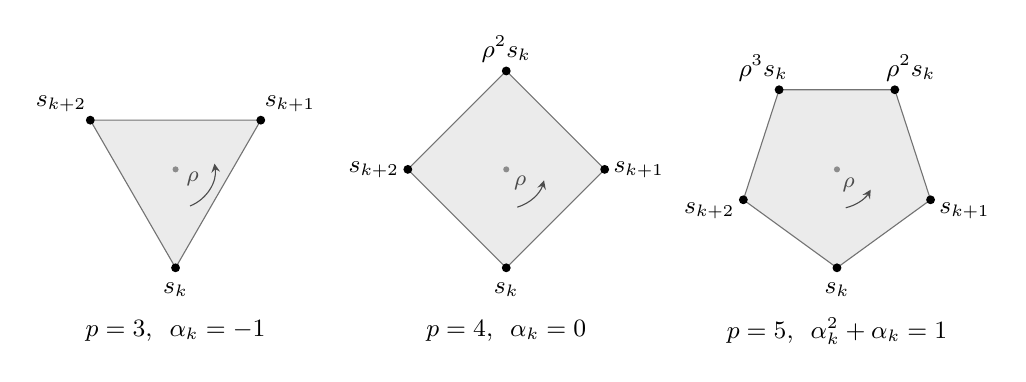
\begin{tikzpicture}[x=1cm, y=1cm, >=stealth, every node/.style={font=\small}]
\foreach \p/\dx/\al in {3/0/{\alpha_k = -1}, 4/4.2/{\alpha_k = 0}, 5/8.4/{\alpha_k^2 + \alpha_k = 1}} {
  \begin{scope}[xshift=\dx cm]
  \pgfmathsetmacro{\stp}{360/\p}
  \pgfmathsetmacro{\anA}{90+\stp}
  \pgfmathsetmacro{\anB}{90-\stp}
  \fill[black!8] (-90:1.25) \foreach \j in {1,...,\p} { -- ({-90+\j*\stp}:1.25) } -- cycle;
  \draw[black!55] (-90:1.25) \foreach \j in {1,...,\p} { -- ({-90+\j*\stp}:1.25) } -- cycle;
  \fill[black!45] (0,0) circle (1.1pt);
  \draw[->, black!70] ({-90+0.18*\stp}:0.5) arc[start angle={-90+0.18*\stp}, end angle={-90+0.82*\stp}, radius=0.5];
  \node[black!70] at ({-90+0.5*\stp}:0.25) {\footnotesize $\rho$};
  \foreach \j in {1,...,\p} \fill ({-90+\j*\stp}:1.25) circle (1.6pt);
  \node[below=2pt] at (-90:1.25) {$s_k$};
  \node[anchor=\anA, inner sep=3pt] at ({-90+\stp}:1.25) {$s_{k+1}$};
  \node[anchor=\anB, inner sep=3pt] at ({-90-\stp}:1.25) {$s_{k+2}$};
  \node at (0,-2.05) {$p = \p$, \ $\al$};
  \end{scope}
}
\node[anchor=south, inner sep=3pt] at ([shift={(4.2,0)}]90:1.25) {$\rho^2 s_k$};
\node[anchor=234, inner sep=3pt] at ([shift={(8.4,0)}]54:1.25) {$\rho^2 s_k$};
\node[anchor=306, inner sep=3pt] at ([shift={(8.4,0)}]126:1.25) {$\rho^3 s_k$};
\end{tikzpicture}
\caption{L'orbite de $s_k$ sous $\rho = \sigma_k\sigma_{k+1}$ dans le plan affine $s_k + W$, sur $\mathbf R$, dans une coordonnée affine où la partie linéaire de $\rho$ est une rotation. Le centre est le point fixe de $\rho$ dans ce plan. Pour $p = 3$, $\rho^2 s_k = s_{k+2}$. L'autre racine de $\alpha^2 + \alpha - 1$, $-(1 + \sqrt 5)/2 = 2\cos(4\pi/5)$, donne la rotation d'angle $4\pi/5$ et le pentagone étoilé.}
\label{fig:70-ordres}
\end{figure}

\begin{remarque}
Voir \texttt{usig\_mul\_self}, \texttt{usig\_comm}, \texttt{sum\_usig}, \texttt{rho\_cubic}, \texttt{orderOf\_rho\_eq\_three}, \texttt{orderOf\_rho\_eq\_four} et \texttt{orderOf\_rho\_eq\_five} dans \href{\leanblob/Folder70.lean}{\texttt{Folder70.lean}}. La lecture démontre le critère sur un corps où $p$ est inversible ; pour $p = 3$, $4$, $5$, les seules valeurs des polytopes réguliers finis, il vaut sur tout anneau, en toute dimension, caractéristiques $2$, $3$ et $5$ comprises. Les générateurs des pages~74 et~75 sont le cas $n = 2$, $(\alpha_0, \alpha_1) = (-1, \alpha)$ (\texttt{usig\_emb}, \texttt{ico\_orderOf}) ; tétraèdre $(-1, -1)$, cube $(0, -1)$, octaèdre $(-1, 0)$ et dodécaèdre $(\alpha, -1)$ sont les autres solides de Platon, et l'autre racine de $\alpha^2 + \alpha - 1$, celle des polyèdres étoilés de la page~69, vérifie les mêmes identités. Ne sont pas démontrés : le critère pour $p$ quelconque, qui demande le polynôme minimal de $2\cos(2\pi/p)$, et le passage de la définition d'une réalisation régulière à la forme normale (pages~7 à~18).
\end{remarque}
